\documentclass[10pt]{beamer}

\usepackage{style-custom}


\title{Use of RG theory in dynamics}
% \subtitle{Colloquio IV anno}
\author[Carmelo Mordini]{Carmelo Mordini}

% \institute[SNS]
% {
%   Scuola Normale Superiore\\
%   %University of Somewhere
%   }
\date{\small{Settembre 2014}}


% % Delete this, if you do not want the table of contents to pop up at
% % the beginning of each subsection:
% \AtBeginSubsection[]
% {
%   \begin{frame}<beamer>{Riassunto}
%     \tableofcontents[currentsection,currentsubsection]
%   \end{frame}
% }

% Let's get started


\begin{document}


%\beamertemplatenavigationsymbolsempty

\begin{frame}[plain]
\advance\textwidth2cm
\hsize\textwidth
\columnwidth\textwidth
  \titlepage
\end{frame}


\begin{frame}{Outline}
\transwipe[direction=270]
  \tableofcontents%[pausesections]
  % You might wish to add the option [pausesections]
\end{frame}

% Section and subsections will appear in the presentation overview
% and table of contents.
\section{Dinamica dissipativa}
\subsection{Equazioni dinamiche}

\begin{frame}{Equazioni dinamiche - I}

Vogliamo studiare la dinamica di un sistema vicino alla transizione di fase, e il modo in cui questo rilassa eventualmente all'equilibrio.

In un modello efficace (\emph{coarse-grained}) del nostro sistema, dobbiamo introdurre delle equazioni cinetiche che descrivano la dissipazione in modo fenomenologico.
\pause
\vskip10pt

\underline{Esempio classico}: moto browniano

\begin{equation*}
 m\ddot{\vec x} = \vec f(x) - \gamma m \dot{\vec x} + \vec \eta(t) \qquad \text{\footnotesize eq. di Langevin}
\end{equation*}

\vskip10pt
overdamping: $\rightarrow \quad \dot p  = -\gamma p + \eta(t)$

scrivi qualcosa che spieghi gamma e eta
magari in un'altra slide
\end{frame}

\begin{frame}{Equazioni dinamiche - II}

Generalizzo ad un sistema con hamiltoniana $\ham [q_i]$

 \begin{equation*}
%     \begin{cases}
%         \dot p_i = -\frac{\partial \ham}{\partial q_i} \equiv v_i\\
%         \dot q_i = \frac{\partial \ham}{\partial p_i} \equiv w_i 
%      \end{cases}
  \dot q_i = \Omega_{ij} \frac{\partial \ham}{\partial q_j} \equiv v_i
    \quad \longrightarrow \quad
    \dot q_i = v_i -\displaystyle \frac{\Gamma_i}{T} \frac{\partial \ham}{\partial q_i} + \zeta_i(t) 
%    \begin{cases}
%         \dot p_i = v_i -\frac{\Gamma_i}{T} \frac{\partial \ham}{\partial p_i} + \zeta(t) \\
%         \dot q = w_i
%      \end{cases}
  \end{equation*}

 \begin{itemize}
 \item<+-> $v_i$ mode-mode coupling fissato dall'hamiltoniana
 \item<+-> $\Gamma$ smorzamento: determina la scala di tempo di dissipazione dell'energia
 
 \item<+-> $\zeta$ rumore gaussiano locale e decorrelato
 \begin{flalign*}
  & \mean{\zeta_i(t)} = 0 \\
  & \mean{\zeta_i (t) \zeta_j (t')} = 2 D_i \ \delta_{ij}\  \delta(t-t') &&
 \end{flalign*}
 
 \end{itemize}

  
\end{frame}

\begin{frame}{Evoluzione della probabilità}
  Con le ipotesi date, la distribuzione di probabilità dello spazio delle fase evolve secondo l'equazione di Fokker - Planck
  
  \begin{equation*}
   \dt P + \sum_i \frac{\partial}{\partial q_i} \left[ v_i - \frac{\Gamma_i}{T} \frac{\partial \ham}{\partial q_i} - D_i \frac{\partial}{\partial q_i} \right] P = 0
  \end{equation*}
\begin{columns}
 \begin{column}{.5\textwidth}
  \begin{figure}
       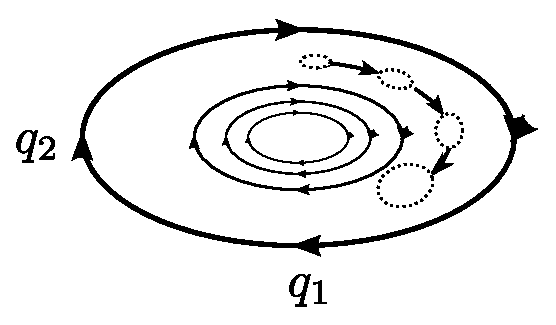
\includegraphics[width=.8\columnwidth]{pics/Oscillator_phase_portrait.eps}
      \end{figure}
  \end{column}
  \hfill
  \begin{column}{.4\textwidth}
   \begin{itemize}
    \item Hamiltonian velocity
    \item Damping
    \item Diffusion
   \end{itemize}
  \end{column}
\end{columns}

\vskip10pt
 per ottenere come soluzione stazionaria la distribuzione di equilibrio $P \propto e^{-\ham/T}$ è necessario soddisfare
 \begin{equation*}
  \Gamma_i = D_i \qquad \qquad \text{\footnotesize relazioni di Einstein}
 \end{equation*}

      
\end{frame}



\section{Funzioni caratteristiche della dinamica}
\subsection{Correlazione e risposta}

% \begin{frame}{Funzioni di correlazione e di risposta}
%   Date le soluzioni $q_i(t)$ si definisce
%  \begin{equation*}
%    C_{ij} (t-t') = \mean{q_i(t)\ q_j(t')}
%  \end{equation*}
%  o in trasformata di Fourier
%  \begin{equation*}
%    2\pi \delta (\omega + \omega') C_{ij}(\omega) = \mean{q_i(\omega)\ q_j(\omega')}
%  \end{equation*}
%  
%  Perturbo l'hamiltoniana con un piccolo campo esterno: $ \ham \rightarrow \ham - \sum_i q_i f_i(t)$\\
% La correzione lineare alle soluzioni si può scrivere come
% \begin{equation*}
%   \mean{q_i(t)} = \sum_j \int dt' \ G_{ij}(t-t')f_j(t') 
% \end{equation*}
% o in trasformata di Fourier
% \begin{equation*}
%   \mean{q_i(\omega)} = \sum_j G_{ij}(\omega)f_j(\omega) 
% \end{equation*}
% \end{frame}


\begin{frame}{Funzione di correlazione}
 Date le soluzioni $q_i(t)$ si definisce
 \begin{equation*}
   C_{ij} (t-t') = \mean{q_i(t)\ q_j(t')}
 \end{equation*}
 o in trasformata di Fourier
 \begin{equation*}
   2\pi \delta (\omega + \omega') C_{ij}(\omega) = \mean{q_i(\omega)\ q_j(\omega')}
 \end{equation*}
La forma di $C(\omega)$ dà informazioni sulla mutua correlazione dei modi $\{i,j\}$. In presenza di dissipazione, mi aspetto che \underline{l'autocorrelazione} $C_{ii}$ decada con una scala temporale tipica di ciascun modo.

\end{frame}

\subsection{Fluttuazione/dissipazione}
\begin{frame}{Funzione di risposta}
Perturbo l'hamiltoniana con un piccolo campo esterno: $ \ham \rightarrow \ham - \sum_i q_i f_i(t)$\\
La correzione lineare alle soluzioni si può scrivere come
\begin{equation*}
  \mean{q_i(t)} = \sum_j \int dt' \ G_{ij}(t-t')f_j(t') 
\end{equation*}
o in trasformata di Fourier
\begin{equation*}
  \mean{q_i(\omega)} = \sum_j G_{ij}(\omega)f_j(\omega) 
\end{equation*}

\pause
\begin{block}{Teorema di fluttuazione-dissipazione}
\begin{equation*}
  C_{ij}(\omega) = \frac{2}{\omega}\im G_{ij}(\omega)
\end{equation*}
  
\end{block}

\end{frame}

\subsection{Toy model}
\begin{frame}{Toy model: teoria di Van Hove}
Hamiltoniana di Ginzburg Laudau, in approssimazione gaussiana

\begin{equation*}
  \ham/T = \frac{1}{2} \sum_{k<\Lambda} (r_0 + ck^2)|\sigma_k|^2 = \frac{1}{2} \sum_{k<\Lambda}{G_0(k)}^{-1}\sigma_k \sigma_{-k} 
 \end{equation*}
 
\begin{equation*}
 \begin{cases}
 \displaystyle \dt{\sigma_k} = -\frac{\Gamma_k}{T}\frac{\partial \ham}{\partial \sigma_{-k}} + \zeta_k(t) = -\Gamma_k {G_0(k)}^{-1} \ \sigma_k + \zeta_k(t)  \\
 \mean{\zeta_k (t) \zeta_q (t')} = 2 \Gamma_k \ \delta_{-kq}\  \delta(t-t') 
 \end{cases}
\end{equation*}

\pause
{\footnotesize
\begin{columns}
 \begin{column}{.5\textwidth}
   La soluzione in trasformata è\\
    \begin{flalign*}
     \sigma_k(\omega) = \frac{\zeta_k(\omega)}{\Gamma_k {G_0(k)}^{-1} - i\omega} &&
    \end{flalign*}
   e mediando sulle $\zeta$ calcolo
   \begin{flalign*}
    C_k(\omega) = \frac{2\Gamma_k}{\left(\Gamma_k {G_0(k)}^{-1}\right)^2 + \omega^2} &&
   \end{flalign*}

 \end{column}

 \begin{column}{.5\textwidth}
  Perturbo $\ham$ con $-\sum_k h_k(t) \sigma_{-k}$\\ La soluzione si sposta in
  \begin{flalign*}
   \mean{\sigma_k(\omega)} = \frac{\Gamma_k \ h_k(\omega)}{\Gamma_k {G_0(k)}^{-1} - i\omega} &&
  \end{flalign*}
  da cui
  \begin{flalign*}
   G_k(\omega) = \frac{\Gamma_k}{\Gamma_k {G_0(k)}^{-1} - i\omega} &&
  \end{flalign*}
 \end{column}

\end{columns}
}

\end{frame}

\begin{frame}{Toy model: teoria di Van Hove}
 \textbf{Remarks}
 \begin{itemize}
  \item Per $\omega = 0$ ritrovo la correlazione statica:\\
  $G(k,\omega = 0) = \int \frac{d\omega}{2\pi} \ C_k(\omega) = \mean{\sigma_{-k}\ \sigma_k} \equiv G_0(k)$
  \item Per ciascun $k$, $C_k$ è una lorentziana di larghezza
  \begin{equation*}
   \displaystyle \tau_k = \frac{G_0(k)}{\Gamma_k} \equiv \frac{1}{\Gamma_k}\ \frac{\xi^2/c}{1+\xi^2 k^2}
  \end{equation*}
  
  \item Per $T \to T_c \quad \left( \xi \to \infty\right) \qquad \Longrightarrow \displaystyle \tau_k \sim \frac{k^{-2}}{\Gamma_k}$
%     \begin{flalign*}
%      \tau_k \sim \frac{k^{-2}}{\Gamma_k} &&
%     \end{flalign*}
 \end{itemize}
 Il tempo di rilassamento \emph{diverge} alla transizione per i modi di alta lunghezza d'onda:\\
%  I modi di alta lunghezza d'onda (responsabili della transizione) hanno tempi di rilassamento divergenti:\\
    \centering \underline{critical slowing down}

\end{frame}



\section{Equazioni di RG}
\subsection{Rinormalizzazione delle equazioni dinamiche}
\begin{frame}{Rinormalizzazione delle equazioni dinamiche}
  Partendo dalle equazioni dinamiche per i modi $\sigma_k$, si applicano i due step già concettualmente definiti nel caso statico:
  \begin{itemize}
   \item[(i)] \emph{Coarse-graining}: elimino dal sistema i modi $\sigma_q$ con $\Lambda/s < q < \Lambda$.\\
   Ovvero, risolvo le equazioni dei $\sigma_q$, le sostituisco nel resto del sistema e medio sul rumore gaussiano $\zeta_q$ dei modi eliminati.
   \item[(ii)] \emph{Scaling \& renormalization}: i modi rimasti vengono riscalati sostituendo
   \begin{flalign*}
    \sigma_k(t) \longmapsto s^{1-\eta/2}\ \sigma_{sk}(s^{-z}t) &&%\Leftrightarrow \sigma_k(\omega) \mapsto s^{1-\eta/2 + z}\ \sigma_{sk}(s^z\omega)&&
   \end{flalign*}

  \end{itemize}

Infine, con il cambio di variabili $\{ t' = s^{-z} t\ ;\ k' = sk \}$\\
si portano le equazioni nella forma di partenza, trovando la legge di trasformazione nello spazio dei parametri allargato $\mu = (v,\ \Gamma,\ \mu_\ham)$. 

\end{frame}

\subsection{Trasformazione delle funzioni}
\begin{frame}{Trasformazione delle funzioni}
% Dopo la trasformazione $\Rightarrow$ le quantità medie dipendenti dai modi che non ho eliminato \underline{rimangono invariate} (non dipendono dalle variabili nel blocco) ed hanno la stessa forma funzionale (la forma delle equazioni è la stessa) [SCRIVILO MEGLIO]
La trasformazione lascia invariate le medie dei modi di alta lunghezza d'onda 
\begin{flalign*}
 \mean{\sigma_k(\omega)\ \sigma_q(\bar\omega)}_\mu = \mean{\sigma'_{k'}(\omega')\ \sigma'_{q'}(\bar\omega')}_{\mu'}  &&
\end{flalign*}
%  \begin{equation*}
%  \begin{cases}
%   \mean{\sigma_k(\omega)\ \sigma_q(\bar\omega)}_\mu = \mean{\sigma'_{k'}(\omega')\ \sigma'_{q'}(\bar\omega')}_{\mu'} \\
%   \sigma'_{k'}(\omega') = s^{1-\eta/2 + z}\ \sigma_{sk}(s^z\omega) \\
%  \end{cases}
%  \end{equation*}

% {\footnotesize
%  \begin{flalign*}
%   & \mean{\sigma_k(\omega)\ \sigma_q(\bar\omega)}_\mu = s^{2-\eta + 2z}\ \mean{\sigma_{sk}(s^z\omega)\ \sigma_{sq}(s^z \bar\omega)}_{R_s \mu} \\
%   & 2\pi \delta(\omega + \bar\omega)\ C(k,\omega,\mu) = 2\pi \delta(s^z(\omega + \bar\omega))\ s^{2-\eta+2z} C(sk,s^z\omega,R_s\mu) &&
%  \end{flalign*}
% }
\begin{block}

\vskip-10pt
\begin{align*}
 & C(k,\omega,\mu) = s^{2-\eta+z}\ C(sk,s^z\omega,R_s\mu)  \\
 & G(k,\omega,\mu) = s^{2-\eta}\ G(sk,s^z\omega,R_s\mu)
\end{align*}

\end{block}
\pause
Al punto critico corrispondente alla transizione di fase, il sistema viene portato da RG in un punto fisso stabile $\mu^*$.

N.B. è necessario che la parte statica dei parametri $\mu_\ham^*$ sia un punto fisso stabile del sistema in equilibrio \emph{(static fixed point)}
\begin{flalign*}
 \begin{cases}
  G(k,\omega,t) = \xi^{2-\eta}\ g(\xi k,\xi^z \omega) \\
  \tau_k(t) = \xi^z\ f(\xi k)\\
  \xi \sim t^{-\nu}
 \end{cases}
 \qquad \text{Si trovano le forme di scala} &&
\end{flalign*}
\end{frame}

\section{Modelli dinamici}
\subsection{Time Dependent Ginzburg Landau}

\begin{frame}{TDGL}
 
 \begin{itemize}
  \item[(i)] senza i termini di mode-mode coupling, le equazioni per i $\sigma_q$ sono disaccoppiate dal resto dei modi
 \[\displaystyle -i\omega \sigma_k = -\frac{\Gamma_k}{r_0 + ck^2}  \ \sigma_k + \zeta_k(\omega) \]

 \begin{flalign*}
  \begin{cases}
   \displaystyle -i\omega \sigma_k = -\frac{\Gamma_k}{r_0 + ck^2}  \ \sigma_k + \zeta_k(\omega)  \\
   \sigma_k(\omega) \mapsto s^{1-\eta/2 + z}\ \sigma_{sk}(s^z\omega) \\
  \end{cases}
&&
 \end{flalign*}
 
 \item[(ii)] con il cambio di variabili $\{ \omega' = s^{z} \omega\ ;\ k' = sk \}$ trovo la forma 
\end{itemize}
\end{frame}

\begin{frame}{Ruolo delle leggi di conservazione}
 
\end{frame}

\end{document}


%%%%%% MAIN DAL COLLOQUIO

% eventualmente da accorciare, ma mi sa ormai di no.
% \input{sections/sez-dinamica2.tex}
% 
% 
% \section{Teoria di campo medio}
% 
% \begin{frame}{Dinamica dei LP}
% 
% \vspace{-.4cm}
% \footnotesize
% 
% \begin{columns}
% \hskip10pt
% \begin{column}{.4\textwidth}
% 
% Se l'ampiezza di interazione tra polaritoni è piccola rispetto allo splitting
% %\( \big(|\omega_p - \omega\lp| \ll \omega\up - \omega\lp \big) \)
% e il pump è accordato vicino al fondo della branca LP, la branca superiore è molto poco eccitata.\\
% La trascuriamo, assieme a tutti i suoi termini nell'hamiltoniana:
% \begin{flalign*}
%   &
%     \begin{cases}
%         \opsi\up \approx 0 \\
%         \opsi_C \approx C\lp \ \opsi\lp \\
%         \opsi_X \approx X\lp \ \opsi\lp
%      \end{cases}
%   \\
%   &\qquad\quad\Downarrow \\
%   &\opsi\lp \approx C\lpsuper{*} \ \opsi_C + X\lpsuper{*} \ \opsi_X
%    \end{flalign*}
%    \end{column}
%     \begin{column}{.6\textwidth}
%       \begin{figure}
%        \includegraphics[scale=.25]{pics/LP_pump.png}
%       \end{figure}
%   \end{column}
%  \end{columns}
% 
% \normalsize
% \begin{align*}
%   \ham = \ \hbar \intr & \opsi\lpsuper{\dagger} \, \big[ \omega\lp(-i\nabla) \big]\, \opsi\lpsuper{} + \frac{g\lp}{2} \opsi\lpsuper{\dagger}  \opsi\lpsuper{\dagger} \displaystyle\opsi\lpsuper{}  \opsi\lpsuper{} \\
%         &+ \left( i F_p e^{ik_p r -i\omega_p t} \ \opsi\lpsuper{\dagger} + \hc \right)
% \end{align*}
% 
% \end{frame}
% 
% 
% \subsection{Gross-Pitaevskii}
% \begin{frame}{Driven Dissipative GPE}
% Mean Field: $\displaystyle \qquad\opsi\lp \longmapsto \left<\opsi\lp\right> \equiv \psi\lp$
% % \[ i\hbar \partial_t \trcurl{\rho \opsi\lp} \approx i\hbar \partial_t \,\psi\lp
% % \]
% 
% %{\centering
% \vspace{5pt}{\footnotesize La sostituzione è esatta per i termini lineari, approssimata per l'interazione:}
% \begin{equation*}
%   \begin{cases}
%              \left< \opsi^\dagger \opsi\, \opsi \right> \approx |\psi|^2 \psi \\
%              \omega\lp (k) \approx {\omega\lp}^0 + \displaystyle\frac{\hbar k^2}{2m\lp} \\
%            \end{cases}
% \end{equation*}
% 
%             
% % ddGPE
% \ovalbox{
% \begin{minipage}{\textwidth}
%  \[
%  i\partial_t \, \psi\lp = \left[ \omega\lp (-i\nabla) + g\lp |\psi\lp|^2 - i \frac{\gamma\lp}{2} \right]\, \psi\lp + i F_p e^{ik_pr - \omega_p t}
%  \]
%  \vskip0pt
% \end{minipage}
% }
% 
% \begin{flalign*}
%  \begin{cases}
%   m\lp = m_C/|C\lp|^2 \qquad &g\lp = |X\lp|^2 \,g_X + |C\lp|^2 \,g_C \\
%   \gamma\lp = |C\lp|^2 \gamma_{{\scriptscriptstyle rad}} \qquad &F_p = C\lp\, \eta E_{inc}
%  \end{cases}
%  &&
% \end{flalign*}
% 
% \end{frame}
% 
% \subsection{Stato stazionario}
% 
% \begin{frame}{Stato stazionario}
% %\input{pandabear.tex}
% Soluzione stazionaria: \( \psi\lpsuper{0}(r,t) = \psi\sts \ e^{ik_pr - i\omega_p t}  \leftarrow\) \alert{phase locking}
% 
% \[
%  \left( \omega_p - \omega\lp (k_p) - g\lp |\psi\sts|^2 + i \frac{\gamma\lp}{2} \right)\, \psi\sts = i F_p
% \]
% 
% La stabilità delle soluzioni si valuta linearizzando attorno alla soluzione $\psi\lpsuper{0}$, e dipende dall'intensità del laser di pump e dal detuning \(\Delta \omega_p = \omega_p - \omega\lp(k_p)\):
% % \begin{figure}
% % \includegraphics[width=\textwidth]{pics/Shapevspump-and-Spectra.png}
% % \end{figure}
% \begin{columns}[t]
%  \begin{column}{.5\textwidth}
%   \begin{figure}
%    \includegraphics[width=\columnwidth]{pics/Shapevspump.png}
%    %\smallcaption{\(\Delta\omega_p <0\) (top) vs \(\Delta\omega_p >0\) (bottom)}
%   \end{figure}
% 
%  \end{column}
% 
%  \begin{column}{.5\textwidth}
%   \begin{figure}
%    \includegraphics[width=\columnwidth]{pics/Spectra.png}
%   % \smallcaption{Spettro di Bogoliubov nei due casi}
%   \end{figure}
%  \end{column}
% 
% \end{columns}
% \let\thefootnote\relax\footnote{\scriptsize Grafici e simulazioni da  Carusotto, Ciuti, \emph{P.R.L.} \textbf{93}, 16 (2004) e\\ \hspace{.55cm}Ciuti, Carusotto, \emph{Phys. Stat. Sol.} \textbf{242}, 11 (2005)}
% 
% \end{frame}
% 
% \subsection{Spettro delle eccitazioni}
% 
% \begin{frame}{Spettro delle eccitazioni}
% Soluzione stazionaria: \( \psi\lp(r,t) = \psi\sts e^{ik_pr - i\omega_p t} + \delta\psi (r,t)\)\\
% Al I ordine in \(\delta\psi\), lo spettro delle eccitazioni (modi di Bogoliubov) si ricava con un procedimento analogo al caso di un gas di bosoni all'equilibrio
% {\footnotesize
% \begin{flalign*}
%  \bvec{\delta \psi} = {\big( \delta\psi \; , \; {\delta\psi}^* \big)}^T \\
%  \\
%  i \partial_t\, \bvec{\delta\psi} = \mathcal{L}\bog \cdot \bvec{\delta\psi}
%  \end{flalign*}
% 
% 
% }
% % {\footnotesize
% % \[
% %  \begin{pmatrix}
% %   \omega\lp (k) + 2 g\lp |\psi\sts|^2 -i\frac{\gamma\lp (k)}{2}       &\hspace{-1cm}  g\lp{\psi\sts}^2 \\
% %   \\
% %   \\ \hspace{-1.8cm}- g\lp{{\psi\sts}^*}^2    & \hspace{-1.8cm}       2\omega_p -\left(\omega\lp (2k_p-k) + 2g\lp|\psi\sts|^2\right) -i\frac{\gamma\lp (2k_p-k)}{2}
% %  \end{pmatrix}
% % \]
% % }
% 
% \[
%  \omega\bogsuper{\pm} = \omega_p + \delta k \cdot v_p -i\frac{\gamma\lp}{2} \pm \sqrt{\left(2 g\lp |\psi\sts|^2 + \eta_{\delta k} - \Delta_p\right)\left(\eta_{\delta k} - \Delta_p\right)}
% \]
% \begin{columns}
%   \begin{column}{.5\textwidth}
%     {\footnotesize
% dove i parametri di controllo entrano in
% \begin{flalign*}
%  \begin{cases}
%     \delta k = k-k_p \qquad \eta_{\delta k}= \frac{\hbar {\delta k}^2}{2 m\lp} \\
%     \Delta_p = \omega_p - \omega\lp(k_p) - g\lp |\psi\sts|^2
%  \end{cases}
%  &&
% \end{flalign*}
% }
%   \end{column}
%   \begin{column}{.4\textwidth}
%   \vspace{-15pt}
%     \begin{figure}
%       \includegraphics[width=.8\columnwidth]{pics/Shapevspump-delta.png}
%     \end{figure}
% 
%   \end{column}
% \end{columns}
% 
% \end{frame}
% 
% 
% \section{Superfluidità}
% \begin{frame}{Perturbazione locale}
% \begin{columns}
% 	\begin{column}{.5\textwidth}
% 	  \[
% 	\mathcal{V} = \intr \sum_{j=X,C} V_j(r) \opsi_j^\dagger \opsi_j
% 	  \]
% 	\end{column}
% 	
% 	\begin{column}{.5\textwidth}
% 	    \begin{itemize}
% 	      \item stress meccanico
% 	      \item variazione $\ell_z$
% 	      \item drogaggio
% 	      \item difetti della cavità
% 	    \end{itemize}
% 
% 	\end{column}
% \end{columns}
% \vspace{10pt}
% Potenziale \underline{statico} $\Rightarrow$ eccita solo i modi ad energia $\omega_p$ 
% \vskip20pt
% %   \begin{figure}
% %   \includegraphics[width=.7\textwidth]{pics/potentials.png}
% %   \mycaption{simulazione numerica}
% %   \end{figure}
% \begin{minipage}{\textwidth}
%   I parametri che determinano la risposta del sistema si possono manipolare dall'esterno:
% \begin{itemize}
%   \item $\theta_p \longrightarrow k_p \longrightarrow$ velocità del flusso
%   \item Pump intensity $\longrightarrow$ densità dei polaritoni $\longrightarrow$ interazione
% \end{itemize}
% % \begin{wrapfigure}{l}{.35\textwidth}
% % \includegraphics[width=.1\textwidth]{pics/laser.png}
% % \end{wrapfigure}
% % \begin{columns}
% %   \begin{column}{.5\textwidth}
% %     \begin{figure}
% %       \centering
% %       \includegraphics[height=.3\textheight]{pics/laser.png}
% %     \end{figure}
% % 
% %   \end{column}
% %   \begin{column}{.5\textwidth}
% %     \footnotesize
% %     esperimento
% %   \end{column}
% % 
% % 
% % \end{columns}
% 
% 
% \end{minipage}
% 
%  \end{frame}
% 
% \subsection{Resonant Rayleigh Scattering}
% \begin{frame}{Resonant Rayleigh Scattering}
% Low/off-resonance excitation: interazioni $LP$ trascurabili\\
% Scattering elastico dei singoli polaritoni
% \begin{columns}[t]
%   \begin{column}{.25\textwidth}
%     \begin{figure}
%         \includegraphics[width=\columnwidth]{pics/scattering-RRS-exp.png}
%     \end{figure}
%   \end{column}
%   \begin{column}{.75\textwidth}
%     \begin{figure}
%       \includegraphics[width=\columnwidth]{pics/scattering-RRS-teo.png}
%     \end{figure}
%   \end{column}
% \end{columns}
% \let\thefootnote\relax\footnote{\scriptsize Dati sperimentali da Amo, Lefrère, \emph{Nat. Phys.} \textbf{5} (2009) }
% \end{frame}
% 
% 
% %%%-----------alternative
% \ifnum\videovariable=1
% {
% \input{sections/sez-regimi-video.tex} 
% 
% }
% \else{
% \input{sections/sez-regimi-foto.tex}
% }
% \fi
% 
% % Placing a * after \section means it will not show in the
% % outline or table of contents.
% % 
% % 
% % \section*{Summary}
% % 
% % \begin{frame}{Summary}
% %   Ciao
% % \end{frame}
% % 
% % 
% % 
% % % All of the following is optional and typically not needed.
% % \appendix
% % \section<presentation>*{\appendixname}
% % \subsection<presentation>*{For Further Reading}
% % 
% % \begin{frame}[allowframebreaks]
% %   \frametitle<presentation>{For Further Reading}
% % 
% %   \begin{thebibliography}{10}
% % 
% %   \beamertemplatebookbibitems
% %   % Start with overview books.
% % 
% %   \bibitem{Author1990}
% %     A.~Author.
% %     \newblock {\em Handbook of Everything}.
% %     \newblock Some Press, 1990.
% % 
% % 
% %   \beamertemplatearticlebibitems
% %   % Followed by interesting articles. Keep the list short.
% % 
% %   \bibitem{Someone2000}
% %     S.~Someone.
% %     \newblock On this and that.
% %     \newblock {\em Journal of This and That}, 2(1):50--100,
% %     2000.
% %   \end{thebibliography}
% % \end{frame}
% 
% \end{document}
